\documentclass{article}
\title{Compilation is communication}
\subtitle{An ode to M-x compile.}
\date{2025-10-13}
\modified{2025-10-13}
\keyword{programming}

\begin{document}

\section*
\epigraph{Never show a half-finished job to a fool.}{A Russian proverb}

\begin{figure}[p25,left]
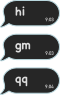
\includegraphics{/images/45-chat.svg}
\end{figure}

However the exchange unfolds,
I'll be impatient.
I want my messages self-contained and coherent.
Instant messaging offers many advantages,
but cultivated, efficient communication isn't one of them.

As software engineers,
we focus on teammates and overlook our even more frequent conversations with tools.
Those interactions have changed drastically over the decades:
Compiling first \textsc{fortran} programs felt like using snail mail,
while starting a modern development environment feels like connecting to an overcrowded Discord server.
In contemporary tooling, the slogan seems to be:
\advice{feedback-hypothesis}{
  Immediate feedback makes us more productive.
}

This claim deserves scrutiny.
I admire
\href{https://en.wikipedia.org/wiki/Seymour_Papert}{Seymour Papert},
\href{https://en.wikipedia.org/wiki/Alan_Kay}{Alan Kay},
and other pioneers of exploratory programming environments.
I applaud \href{https://worrydream.com/}{Bret Victor} and his vision of \href{https://youtu.be/5Q9r-AEzRMA}{Dynamicland}.
Yet, I disable most of my editor's features,
call my batch compiler,
and carefully read its output.
Why would I ignore decades of progress in developer experience?

\section{constant-interaction}{The perils of constant interaction}

First, unsolicited feedback breaks my focus.
Here I am, holding a virtual castle in my mind and trying to will one of its towers into existence,
and here comes an anxiety-inducing squiggly underline.
I interrupt myself to make it go away, and, victorious, observe the castle’s ruins.

IntelliSense-style code completion doesn't bother me
because its suggestions stay relevant and unobtrusive.
However, \textsc{ai} completion tools drain my energy like watching a movie in my native language with mismatching subtitles.
They force my brain to switch from the composition mode (\href{https://en.wikipedia.org/wiki/Frontoparietal_network}{central executive network})
to evaluation mode (\href{https://en.wikipedia.org/wiki/Salience_network}{salience network}) every time I type a word.

Second, I become frustrated when my tools don’t respond promptly.
My attention drifts if the letters I type don't appear on the screen \emph{instantly}
due to my editor cooking something in the background.
I don't mind waiting if my request is inherently slow;
what bothers me is when a tool prioritizes something else over my request.

These points might seem to contradict each other,
as I'm asking for less and more interactivity simultaneously.
What counts, however, is \emph{when} the interaction happens.
I enjoy tools that remain silent until I need them
and respond quickly once summoned.
Two ideas convince me that calmer tool conversations benefit not only my messy mind:
batching and mastery research.

\section{batching}{The power of batching}

Batching is the cornerstone of computer optimization,
and its power goes far beyond the digital world:
\begin{itemize}
\item Henry Ford used batching to build the most efficient production line of his time.
\item Productivity experts, ranging from David Allen to Cal Newport,
recommend time-boxing and batch-processing communications.
\item Prolific writers recommend silencing the inner critic and delaying editing
until the \href{https://blog.reedsy.com/live/draft-zero-sj-watson/}{draft zero} is complete.
\end{itemize}

Steven Pressfield summarized the last point well:
  
\blockquote{
  Let's talk about the actual process—the writing/composing/idea generation process.
  It progresses in two stages: action and reflection.
  Act, reflect. Act, reflect.
  NEVER act and reflect at the same time. [\ldots]
  In writing, ``action'' means putting words on paper.
  ``Reflection'' means evaluating what we have on paper.
  For this first draft,
  we'll go light on reflection and heavy on action.
}{Steven Pressfield, ``Do the Work''}


Writers like Neil Gaiman and J.K. Rowling draft longhand,
partly because paper makes revision hard and nudges them toward action\sidenote{sn-longhand}{
  I draft blog posts longhand if they involve complex arguments.
  Effortless text editing paralyzes me:
  I keep re-editing and restructuring the same few sentences instead of developing my ideas.
}.

Overall, chunking complementary activities works so well
that I separate creative coding from dealing with compiler pedantry.

\section{expertise}{Tools and expertise}

The time I can go without the compiler's feedback is proportional to my expertise in the language and the codebase.
At the height of my C++ abilities,
I could write a 100 \textsc{loc} self-contained program involving template meta-programming that would compile on the first try.
On the other hand,
I can't write a one-liner in an unfamiliar language without a dozen interactions with its compiler or interpreter.

As people progress from novices to experts,
their relationship with feedback changes.
Feedback is vital for achieving proficiency,
but a master internalizes the system so well that the need for external input diminishes;
masters generate their own feedback.
That's why you notice when you mistype your password before you hit the enter key:
you've typed the symbols correctly so many times that you've internalized the feel of it.

No wonder experts and novices prefer different tools and workflows.
Experts aren't fond of graphical menus; they prefer shortcuts.
Many outstanding programmers use a bare text editor.
Edward Kmett is a good example:
He authored over a hundred popular Haskell packages using a minimal Vim setup
before he added \href{https://neovim.io/doc/user/tagsrch.html}{\code{tags} files} to his workflow\sidenote{sn-kmett-live}{
  The \href{https://youtu.be/hIZxTQP1ifo?si=MliJIlho6h7Ybng-&t=2827}{Type Classes vs. the World} talk has a good example of him doing live programming.
}.
Aaron Hsu sometimes delves deeper and \href{https://www.sacrideo.us/paper-is-dead-long-live-paper-programming/}{programs on paper}.
André Bensoussan \href{https://www.multicians.org/andre.html}{wrote one of Multics's subsystems} on paper.

Christof van Nimwegen's thesis,
\href{https://dspace.library.uu.nl/bitstream/handle/1874/26875/nimwegen.pdf}{The paradox of the guided user: assistance can be counter-effective},
suggests that the connection between mastery and minimalistic tools also works in the other direction:
Simple tools foster deeper understanding.
Nimwegen asked two groups of people to solve a tricky logic puzzle on a computer.
The first group enjoyed helpful interactive software that suggested legal moves;
the second group was given only bare-bones software that provided no hints.
The first group initially made more progress,
but the second group quickly caught up and took over,
demonstrating ``more focus, more direct and economical solutions, better strategies, and better imprinting of knowledge.''

I don't imply that interactive tools are inferior and that \href{https://xkcd.com/378/}{real programmers use butterflies}.
If the task is novel or if the language is particularly demanding,
even experts will struggle without appropriate tools.
A tool isn't inherently good or bad;
we prefer different tools depending on our proficiency
and the task's cognitive load demands.

\href{https://en.wikipedia.org/wiki/John_Carmack}{John Carmack},
one of the most influential programmers in history,
relies heavily on \textsc{ide}s and visual debuggers:

\blockquote{
  The first thing I do after writing code is set a breakpoint and step through the function.
}{
  John Carmack, \href{https://www.youtube.com/watch?v=tzr7hRXcwkw}{interview with Lex Fridman}
}
This approach is common among game developers and graphics programmers,
where the ``right'' results don't follow logically from the first principles.
The \href{https://tomorrowcorporation.com/}{Tomorrow Corporation} team
\href{https://www.youtube.com/watch?v=72y2EC5fkcE}{built their own programming language and environment}
to facilitate live experimentation and debugging,
and the \href{https://loglog.games/}{LogLog Games} studio \href{https://loglog.games/blog/leaving-rust-gamedev/#hot-reloading-is-more-important-for-iteration-speed-than-people-give-it-credit-for}{treats hot reload as the top priority} when picking their technology stack.

Note, however, the batching aspect of John's workflow:
he switches between composition and refinement.
Interactive debuggers don't interfere with authoring;
they fade away when they aren't needed.

\section{my-workflow}{My workflow}

I separate my work into two phases: authoring and cleaning up.
During the authoring phase,
I write and refactor code, design interfaces, and write documentation.
Once I reach a meaningful milestone,
I enter the cleaning phase in which I run the compiler and linters and address their findings.
This phase also serves as a natural rest point before I return to the demanding authoring mode.

The first phase doesn't need much tooling beyond regular text editing and basic \textsc{lsp} support.
The second phase hinges on the concept of the \emph{error list}.
Batch tools report issues,
my editor parses them into a navigable list,
and I refresh it after each pass until it's empty.

Emacs's \href{https://www.gnu.org/software/emacs/manual/html_node/emacs/Compilation.html}{compilation mode} is the most convenient implementation of my workflow.
Running a compiler populates Emacs's global error list that I can navigate with hotkeys
(\code{M-g n} goes to the next error on the list, \code{M-g p}---to the previous).
Typing \code{g} in the compilation buffer reruns the build and refreshes the list.
The build process is interactive and asynchronous.
The compilation output is a regular buffer:
I can open it in a vertical split, so even long-winded errors fit on the screen.

\begin{figure}
  \marginnote{mn-emacs-compile}{
    The interface of Emacs's compilation mode (the right buffer in the vertical split).
  }
  \includegraphics{/images/45-emacs-compile.webp}
\end{figure}

Vim's \href{https://neovim.io/doc/user/quickfix.html}{quickfix} list comes as a close second.
Vim's \code{:make} command is synchronous
(the \href{https://github.com/tpope/vim-dispatch}{vim-dispatch} plugin addresses this shortcoming),
requires more configuration,
and is somewhat less flexible
(the quickfix window is stubborn in its preference for horizontal splits, which can make long error messages unreadable),
but it's also packed with more features,
such as error list history (see \code{:cnewer} and \code{:colder})
and batch editing on quickfix entries (see \code{:cdo} and \code{:cfdo}).
Typing \code{]q} or \code{[q} shifts the focus to the next/previous list entry.

\begin{figure}
  \marginnote{mn-nvim-quickfix}{
    The interface of Neovim's quickfix feature (the bottom buffer in the horizontal split).
  }
  \includegraphics{/images/45-nvim-quickfix.webp}
\end{figure}

Many other editors support this workflow.
For example, \href{https://code.visualstudio.com/}{VS Code} can run external tools
as \href{https://code.visualstudio.com/docs/debugtest/tasks}{tasks}
and populate the error list via \href{https://code.visualstudio.com/docs/debugtest/tasks#_defining-a-problem-matcher}{problem matchers},
but that setup creates enough friction that I always return to bureaucracy-free Emacs.

\section{conclusion}{Conclusion}

A programmer's interaction with a tool is a conversation.
Most modern tools treat this conversation as instant messaging,
trading depth for interactivity,
interrupting the natural pace of discussion,
and trying to finish programmers' sentences for them.

Interactive tools are a great asset when they don't interfere with authoring;
they can help us stay more focused and engaged for longer.
Conversations need pauses. Music is the space between the notes.

\end{document}
